\hyt{dvakrat}
\song{Dvakrát}
\note{capo 3}
\vspace{5mm}

\intro{

\vspace{-25pt}
\hspace{20pt}	
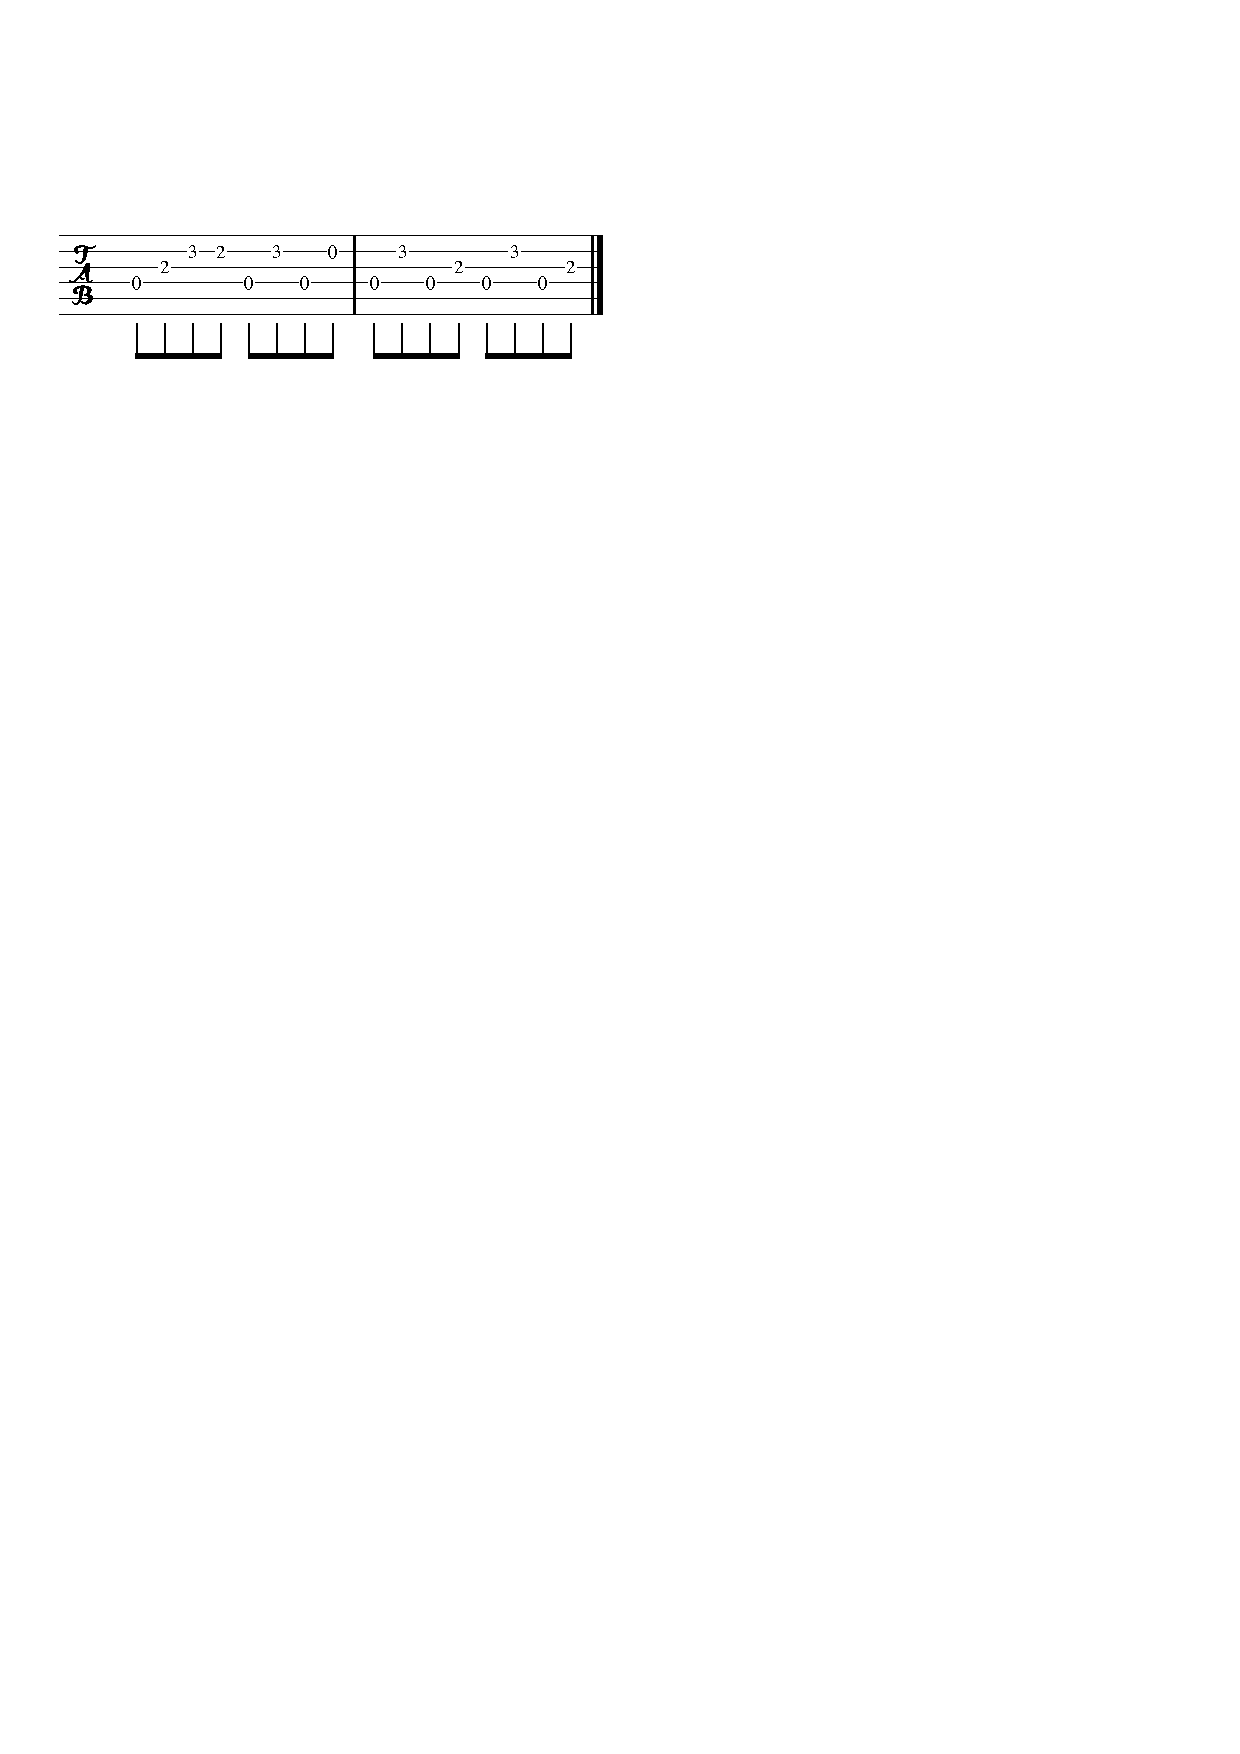
\includegraphics[width=\linewidth]{scores/dvakrat.pdf}
}
\ns

\vers{1}{
\chord{D}Dvakrát dvě deci \chord{G}přede mě \chord{A}postavil \chord{D}pán,\\
musel si přeci všimnout, že jsem tu sám.\\
Dvakrát se uklonil, dvakrát poděkoval,\\
skupina spustila \uv{Andulko Šafářova}
}
\ns

\vers{2}{
Ach, to je muzika, až se mi \textsuperscript{\emph{(ještě,}} srdce \textsuperscript{\emph{že na)}} svírá,\\
dvojitý Nelson dvakrát se neumírá,\\
od stolu vstávají ti, co tu nejsou sami, \textsuperscript{\emph{(tak)}}\\
proč stojíš u mě, dívenko s květinami?
}
\ns

\vers{3}{
Holky rty špulí na stébla v citrokolách,\\
všechny jsou v stejném -- copánky, mašle, volán,\\
všechny si naráz dávají hádat z dlaně,\\
ta, co je nejblíž, vypadá odhodlaně.
}

\refrainn{1}{
A tak \chord{G}provlékám \chord{G\bas{F}}skrz to hlu\chord{C}ché \chord{E\7}\nc \chord{A}velblouda i \chord{A\7}jehlu u\chord{D}chem,\chord{D\7}\\
to jsem \chord{G}netušil, \chord{G\bas{F}}že je to tak \chord{E\7}náramně jednodu\chord{A7}ché. \chord{G}
}

\vers{4}{
To je ta pravá chvíle pro autogramy,\\
plaše se sklání a voní fialkami,\\
raději jděte mi z očí, tajemná Eurydiko,\\
nějak dnes nesnáším pohled na krev a mlíko.
}
\ns

\vers{5}{
Samoto, samoto, laskavá domovino,\\
syn se ti vrátil, tak ještě dvakrát víno,\\
ať ještě chvíli je všechno tak hezky sudé,\\
ať se smím loudat pár kroků za osudem.
}
\vspace{-4mm}

\refrainn{2}{
A ona ať oči klopí, ať se v těch hlubinách neutopím.\\
Kéž bych tak neviděl, neslyšel, co nikdy, nikdy nepochopím.
}
\vspace{-4mm}

\vers{6}{
Ještě se třpytí, jak slza na kameni\\
a už tu není, zmizela bez loučení,\\
ani ten v černém dvakrát si neví rady,\\
pán si přál platit, zvlášť nebo dohromady?
}
\newpage
